\chapter{Cadre institutionnel de l'\'etude }
\section*{Introduction}
Le cursus en Master 2, est sanctionn\'e par la r\'edaction et la soutenance d'un m\'emoire de fin de formation. Afin de valider notre dipl\^ome, il est n\'ecessaire d'effectuer un stage, au cours duquel nos acquis th\'eoriques seront r\'einvestis pour solutionner des probl\`emes m\'etiers. Ce chapitre pr\'esente le cadre institutionnel de notre stage et le sujet qui nous a \'et\'e confi\'e. Apr\`es une pr\'esentation de la structure d'accueil et de la probl\'ematique, nous allons exposer le cahier de charges ainsi que la m\'ethode de travail adopt\'ee.

\section{Cadre contextuel}

\subsection{Pr\'esentation de l'organisme d'accueil}
\subsubsection{\textbf{Sanlam Group}}
Fondée en 1918 en tant que compagnie d’assurance vie, Sanlam (South African National Life Assurance Company Limited) est aujourd’hui un groupe leader des services financiers diversifiés, basé en Afrique du Sud. Il déploie ses activités à travers l’ensemble du continent africain ainsi qu’en Malaisie, aux Etats-Unis, en France, en Suisse, en Inde et en Australie. Groupe financier de référence coté à la bourse de Johannesburg, Sanlam offre des solutions financières complètes et personnalisées dans tous les segments du marché, à travers ses cinq (5) pôles d’activités : Sanlam Personal Finance, Sanlam Pan-Africa, Sanlam Investments, Sanlam Corporate et Santam (South African National Trust and Assurance Company Limited).
\begin{figure}[!h]
  \caption{Organigramme de Sanlam Group}  \label{fig:xray}
  \begin{center}
  \hspace*{-1.0in}
  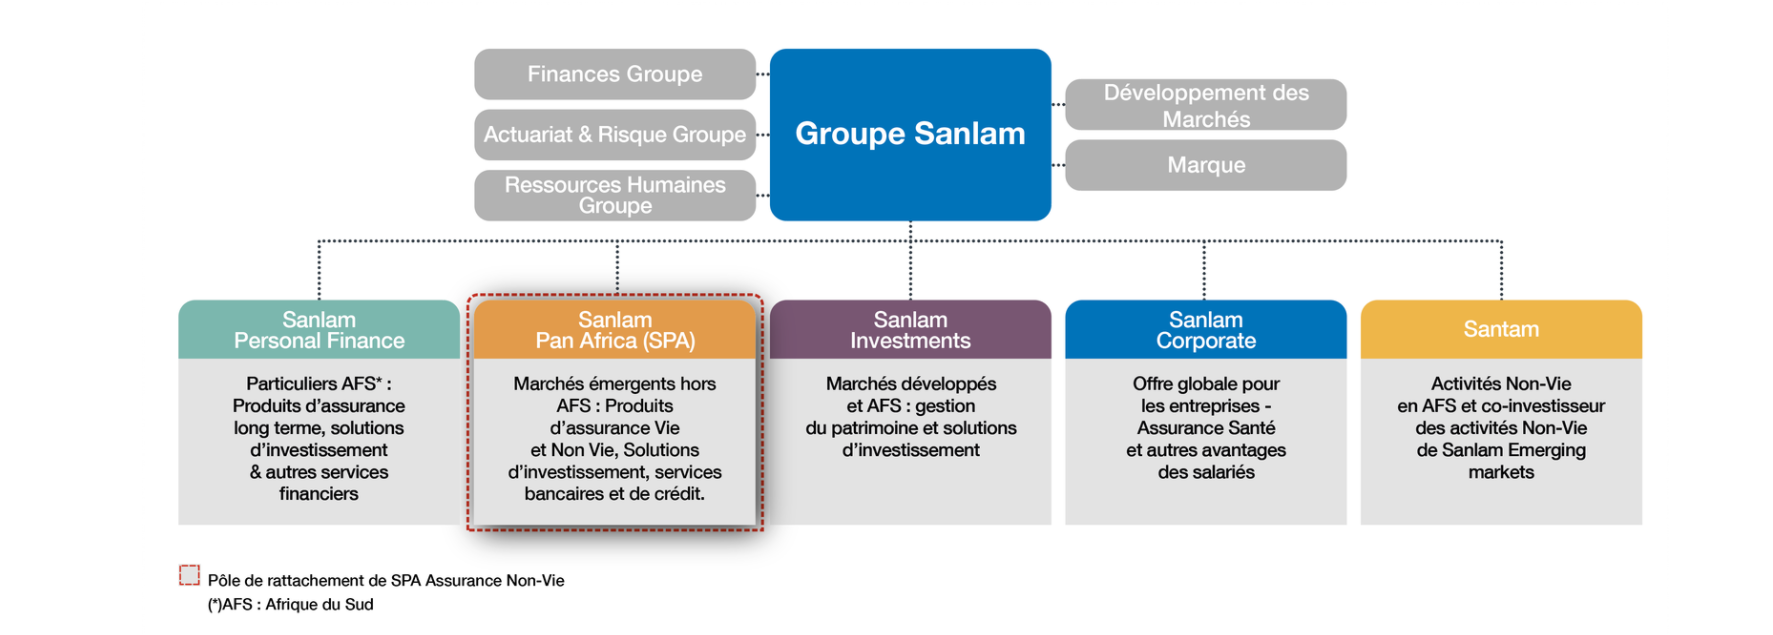
\includegraphics[scale=0.30]{Static/Organigramme.png} 
  \end{center}
\end{figure}
\\

C'est l'un des plus grands groupes d'assurance ayant une couverture internationale, dans le monde, en termes de présence, avec une présence directe et indirecte dans quarante-quatre (44) pays, à l'exception de l'Afrique du Sud. Sanlam Group, fournit plus précisément des solutions et produits financiers aux particuliers et aux entreprises \`a savoir :
\begin{itemize}[parsep=0cm,itemsep=0cm]
\item la planification financière et conseil;
\item l'assurance vie et non vie, la r\'eassurance;
\item la gestion de patrimoine, interm\'ediaire boursier;
\item la gestion des fonds (pensions, retraites,...).
\end{itemize}
%\vspace {0.5cm}
%\paragraph{}

\`A  Sanlam Group, on développe une vision portée sur la création de valeur pour le client, placé au cœur de toute stratégie de développement. Par ailleurs, il ambitionne de consolider ses positions sur le segment des solutions d’investissement sur les marchés développés. 
%Sa vision strat\'egique est de créer de la valeur durable pour toutes les parties prenantes. Elle se d\'ecline sur 3 axes principaux:
%\begin{itemize}[parsep=0cm,itemsep=0cm]
%\item pour l'Afrique du Sud : \^etre leader dans la gestion de patrimoine, le management et la protection;
%\item pour l'Afrique, l'Inde, la Malaisie et le Liban : \^etre un Groupe de services financiers panafricain de premier plan avec une présence significative en Inde et en Malaisie;
%\item pour les march\'es d\'evelopp\'es : se positionner sur la niche de gestion du patrimoine et de placements sur des marchés développés spécifiques.
%\end{itemize}
%\vspace {0.5cm}
Au sein du Groupe, notre stage s'est d\'eroul\'e au p\^ole Sanlam Pan-Africa. 
\subsubsection{\textbf{Sanlam Pan-Africa}}
\acrfull{spa} est le pôle d’activités de Sanlam Group opérant sur les marchés émergents (hors Afrique du Sud). \acrshort{spa} assure ainsi le développement et le déploiement d’une gamme diversifiée de produits d’assurance Vie et Non-Vie, ainsi que des solutions d’investissement, des services bancaires et de crédit à la consommation, la bancassurance, la gestion d’actifs et des produits d’assurances Non-Vie spécialisées pour l’Afrique, l’Inde, la Malaisie et le Liban. L’Afrique est aujourd’hui une composante fondamentale de la vision de Sanlam Group, d’où la mission stratégique fondamentale dévolue à \acrshort{spa} : ériger un groupe de services financiers panafricain de premier plan. Disposant de la première empreinte panafricaine qui lui garantit un rayonnement continental unique, \acrshort{spa} se positionne notamment en tant que partenaire privilégié des multinationales et autres réseaux de distribution. Au sein de SPA, nous avons effectu\'e notre stage \`a la \acrfull{df} de Saham Maroc, afin de b\'en\'eficier d'un suivi ad\'equat.

\subsubsection{\textbf{Digital Factory }} 
La \acrlong{df}, est un espace où des experts en digital travaillent et r\'efl\'echissent sur l’accélération de la transformation digitale et l’élaboration de solutions pour une expérience client optimale. La \acrshort{df} se veut \textit{customer centric} et proactive pour livrer des produits efficaces et utiles
pour les métiers en un temps record. Pour cela, en plus des compétences recrutées et de leurs expériences, elle mise sur une approche organisationnelle du travail : l’agilité à travers la méthode Scrum\footnote{concept d\'efini \`a les section 1.2.3}. Grâce à la \acrlong{df}, Saham Assurance Maroc innove sur des produits qu’elle lance au fur et à mesure. Elle comprend plusieurs \'equipes constituées aussi bien de d\'eveloppeurs, d'\acrfull{ui_ux} designers, de \textit{data scientists}, \textit{data engineers}, \textit{data architects}, de coach agile...
\\

En raison des conditions sanitaires, notre stage s'est effectu\'e physiquement \`a Colina Participations (qui est la \textit{holding} du groupe Sanlam d\'etenant les parts dans les diff\'erentes filiales en Afrique hors Maroc et Afrique du Sud) mais virtuellement (\`a distance) \`a la \acrlong{df}. Nous avons \'et\'e suivis et encadr\'es dans un environnement convivial et agile. Ce stage nous a permis d'\^etre beaucoup plus autonome et de pouvoir transformer les besoins m\'etiers ainsi que les contraintes \textit{business} en r\'ealisations techniques.  


\subsection{Qualit\'e des donn\'ees en assurance}
L'assurance est un secteur qui a pour principale mission de fournir une prestation lors de la survenance d'un événement incertain et aléatoire souvent appelé 'risque'. La prestation, généralement financière, peut être destinée à un individu, une association ou une entreprise, en échange de la perception d'une cotisation ou prime. L'assurance se d\'efinit aussi comme \'etant une op\'eration par laquelle l'assur\'e transf\`ere ses risques \`a l'assureur en contrepartie du paiement d'une prime. 
\\

Bien qu'\'etant un secteur majeur dans les activit\'es \'economiques d'un pays, l'assurance se distingue par l'inversion du cycle de production. En effet, il est impossible aux compagnies de savoir avec certitude, combien la prestation qu’elles vendent leur coûtera, la prime étant payée par le client avant l'indemnisation. Ainsi, pour fixer le montant de sa prime ou calculer les provisions, l’assureur ne peut se baser que sur des études statistiques lui permettant de se faire une idée de combien lui coûtera sa prestation en analysant par exemple le taux de sinistralité et le co\^ut moyen des sinistres ant\'erieurs. Cela ne donne pas pour autant la certitude qu’il n’aura pas à faire face à des sinistres majeurs (en termes de fr\'equence ou de co\^ut). La fiabilité des systèmes d’information et la qualité des données doivent alors constituer un objectif permanent, dans un environnement  incertain et malgr\'e tout concurrentiel.  \\
 

Ce sujet est donc au cœur du modèle d’affaires des assureurs. La parfaite maîtrise des systèmes d’information et des dispositifs de sécurité sont des leviers stratégiques voire vitaux pour maintenir une position de leader dans le domaine. Elle permet notamment de  : 

\begin{itemize}[parsep=0cm,itemsep=0cm]
\item se distinguer en termes de tarification, gr\^ace à une segmentation plus efficiente avec la possibilité de créer de nouvelles offres ;
\item se distinguer en termes de gestion des risques, par une optimisation des couvertures et des provisions;
\item mettre en place de meilleurs systèmes de détection des fraudes.
\end{itemize}    
L’enjeu est crucial à tous les niveaux : que ce soit pour une bonne appréhension des risques, pour mener les études actuarielles, réaliser les tarifications, évaluer les provisions ou fiabiliser les modèles, etc. \\

Les organismes assureurs sont donc, sensibles aux gains de productivité espérés qui pourront se traduire dans la compétition avec les autres acteurs du marché. De ce fait, les défauts de qualité des données peuvent constituer un frein à la compétitivité du groupe face aux concurrents et s’avérer être coûteux pour plusieurs raisons. Tout d’abord, ils (les d\'efauts de qualit\'e) rendent plus difficiles l’ensemble des travaux de production puisqu’ils complexifient les traitements. De plus, des données de mauvaise qualité sont susceptibles de conduire à une dégradation ou à l’allongement des travaux et des analyses qui en résultent. Enfin, elles impactent la qualit\'e des services offerts aux clients. En effet, selon une étude du \acrfull{mit} (MIT, 2017) \cite{MIT2017}, la non-qualité occasionne une perte d'argent estimée entre 15\% et 25\% du chiffre d’affaires total de la plupart des entreprises. Environ 20 ans plus t\^ot, cette perte s'\'evalue \`a 5\% - 10\% du revenu des entreprises \cite{Techno7}. De m\^eme, dans \cite{efrontech},  l’institut Gartner estime que plus de 25\% des données des plus grandes entreprises mondiales sont erronées et précise \'egalement qu'un tel probl\`eme n’a pas une conséquence informatique mais plut\^ot une cons\'equence commerciale, se chiffrant en millions de devises mon\'etaires. Cette perte représentant environ un quart des revenus, s’explique par les mauvais choix stratégiques opérés à partir d’informations erronées, mais aussi par le temps perdu par les services informatiques à traiter ces données inexactes:  contr\^oles, corrections et maintenances. Ramener au secteur de l'assurance, une non-qualit\'e des donn\'ees peut nuire aux décisions prises s’agissant aussi bien des exigences r\'eglementaires que des choix strat\'egiques de l’entreprise (mauvaise interprétation de la situation actuelle par exemple) \cite{Axysweb_Consequences}. Prendre une décision à partir de mauvaises informations affecte l’entreprise, ses clients ou ses partenaires.
\\

La d\'efinition d'une bonne strat\'egie de gouvernance des données est un sujet qui prend de l’importance dans les entreprises et les administrations. Il urge alors de se pencher plus s\'erieusement sur cette probl\'ematique tout en prenant en compte le contexte technologique. Il est impensable que les données de l’assureur ne soient pas à la hauteur des attentes. Une défaillance sur ce volet-là a de lourdes conséquences. Point d'ancrage de toute strat\'egie de gouvernance des donn\'ees, la mise en place d'un projet de qualit\'e des donn\'ees requiert quelques interrogations: qu'est-ce que la qualit\'e des donn\'ees et comment la mesurer? Quels sont les diff\'erents outils de qualit\'e des donn\'ees et quels sont les avantages qu'offre Apache Griffin vis-\`a-vis de ces derniers? Comment corriger les probl\`emes de qualit\'e des donn\'ees d\'etect\'es?


%%\section{M\'ethodologie de recherche}

%Lorem ipsum dolor sit amet, consectetur adipiscing elit. In maximus imperdiet mauris, eu tempor diam pulvinar ut. Etiam dignissim ultrices eros, pellentesque feugiat libero pharetra sit amet. Praesent et lacinia augue. Sed eget mi sit amet elit fringilla commodo. Maecenas finibus est velit, vitae commodo ante dictum at. Fusce nec nibh non mauris sollicitudin tempor vel sed ligula. Donec ac dictum risus. Maecenas consectetur turpis eget egestas faucibus. Vestibulum pretium suscipit diam, vitae feugiat ex tempus ut. Proin elementum faucibus est non porta. Aliquam sed sapien est. 
%\subsection{Objectifs }
%\subsection{Questions de recherche}
%\subsection{M\'ethode de recherche}
%\subsection{Valeur du travail}

%\section{\'Etude de l'existant}
%\`A la Digital Factory de Saham Maroc, suite \`a l'absence de moyen de v\'erification de la qualit\'e des donn\'ees, aux incoh\'erences rencontr\'ees dans le calcul des primes et aux difficult\'es dans la r\'ealisation de regroupement fiable, le besoin s'est fait ressentir de mettre en place un outil permettant d'industrialiser la gestion de la qualit\'e des donn\'ees . Cet outil viendra remplacer les tests manuels (SQL) et les explorations effectu\'ees sans industrialisation. 
%\section{Management du projet}

%(Une introduction partielle)

\section{Terms of reference}
The \acrlong{df} has developed a data base in agile mode to modernize and digitalize certain business processes. In order to achieve these objectives and develop new Business Intelligence capabilities at the Group level, it is necessary to :
\begin{itemize}[parsep=0cm,itemsep=0cm]
    \item review the functional and technical architecture in order to make the data base more robust and scalable but also;
    \item implement a data governance program to improve data quality.
\end{itemize}
\subsubsection{\textbf{Overall objective }}
%L'objectif g\'en\'eral est de d\'etecter et de corriger les probl\`emes de qualit\'e de donn\'ees dans le cadre du projet socle de donn\'ees de la Digital Factory. La d\'etection se fera \'a l'aide de l'outil Apache Griffin. Il est de ce fait subdiviser en deux volets : le volet outil et le volet correctif.

The general objective of our subject is to evaluate in a first step with the help of Apache Griffin, the quality of the \acrlong{df}'s data. And then to proceed to a correction of the various detected anomalies. It is thus subdivided into two parts:
a tool component and a detection and correction component.
\subparagraph{\textbf{> Tool component: Specific objectives}} The purpose of this component is to :
\begin{enumerate}[parsep=0cm,itemsep=0cm]
    \item take in hand the data quality audit tool Apache Griffin ;
    \item establish the connection with the different databases;
    \item analyze the perspectives offered by this tool.
\end{enumerate}
\subparagraph{\textbf{> Detection and correction component: Specific objectives}} The aim here is to use the tool to identify the various data quality problems and, if necessary, propose corrective measures. More specifically, it will be necessary to do:
\begin{enumerate}[parsep=0cm,itemsep=0cm]
    \item a review of the different data in the base and detect inconsistencies with the different data and extractions used by the business;
    \item a prioritization of the main fields to be improved;
    \item an implementation of data rectification algorithms when possible ;
    \item possibly an injection of open data to improve the quality of prioritized data.
\end{enumerate}

\section{Analysis of the existing situation}
Data quality auditing at the \acrlong{df} is not a new issue. It was done by means of manual exploration of the data and \acrshort{sql} (\acrlong{sql}) queries. This method did not allow for a real industrialisation of the quality assessment and was carried out after the fact. Indeed, it did not offer the possibility of monitoring the evolution of metrics over time, which is very important in the quality management process. Moreover, the absence of a real upstream verification tool for data quality prevents the preventive detection of irregularities. These inconsistencies are only detected at the data enhancement stage, requiring exploration of the data to identify the sources of irregularity. All this has an impact on the productivity and performance of the company. The idea of working on the exploration of a data quality audit tool is at several levels. Firstly, a tool dedicated to data quality would allow it to be easily integrated into the production chain. Secondly, the choice of the tool should correspond to the requirements of the \acrshort{df} in terms of detection and malleability.
%\subsection{M\'ethode de travail agile}
%La méthode Agile est une méthodologie de gestion de projet. Il s'agit d'une organisation de travail en cycles courts, permettant aux équipes de développement de gérer un produit de manière souple, adaptative et itérative. Pour cela, elle place le client au cœur du projet et s’adapte tout le long  du projet. De plus, au lieu de planifier le projet de A à Z dès le départ, ce qui laisse peu de place aux imprévus, des objectifs courts sont fixés, par exemple à deux ou trois semaines. Le projet est divisé en sous-projets et l’on ne passe au suivant que lorsque le précédent est réglé. Le principal avantage est la flexibilité, la possibilité de s’adapter en fonction des nouvelles exigences du client ou des évolutions du marché. \\
%Il existe en réalité plusieurs méthodes qui ont toutes un point commun : elles découlent toutes du Manifeste Agile. Scrum est aujourd’hui l’approche Agile la plus répandue; il s'agit plus précisément d'un cadre m\'ethodologique plut\^ot que d'une m\'ethode. Elle est d'ailleurs celle impl\'ement\'ee par la \acrshort{df}. De plus, Scrum est une pratique Agile élémentaire qui permet également une mise à l’échelle, autrement dit le déploiement progressif de l’agilité à l’échelle de l’entreprise. 
%Scrum est constitué d'une définition des rôles, de réunions et d'artefacts \cite{Nutcache_agile} \cite{Agiliste_agile}. 
%\subsection{Organisation et planning du projet (d\'ecrire l'impl\'ementation du scrum dans le cadre du projet et les sprints --Not Yet Done)}


\section*{Conclusion}
La \acrlong{df} de Saham Maroc, est un espace où des experts en digital travaillent et réfléchissent sur l’accélération de la transformation digitale et l’élaboration de solutions innovantes dans une approche \textit{data-centric}. Elle a mis en place un programme de gouvernance de donn\'ees afin d'am\'eliorer la qualit\'e des donn\'ees de son socle de donn\'ees. Notre projet porte sur le volet qualit\'e o\`u il s'agira de d\'etecter et de corriger les probl\`emes de qualit\'e. Des donn\'ees de bonne qualit\'e permettront \`a Saham Assurance Maroc de pouvoir se distinguer notamment en termes de tarification et en termes de gestion des risques. Le chapitre suivant fera l'objet d'une pr\'esentation du cadre th\'eorique et m\'ethodologique de notre \'etude.